\documentclass{article}

\usepackage[a4paper]{geometry}
\usepackage{fancyhdr}
\usepackage{graphicx}
\usepackage{listings}
\usepackage{textcomp}
\usepackage{hyperref}
\usepackage{lastpage}
\usepackage{amsmath}
\usepackage{amsfonts}
\usepackage{amssymb}
\usepackage{amsthm}
\usepackage{xltxtra}
\usepackage{fontawesome5}
\usepackage{footnote}
\usepackage[format=plain,justification=centering]{caption}
\makesavenoteenv{table}

\graphicspath{{img/}}

\AddToHook{cmd/section/before}{\newpage}

\newcommand{\Title}{Early Earthquake and Tsunami Warning Viewer}
\newcommand{\Author}{Yicheng Shao (Eason)}
\newcommand{\CandNo}{[1234]}

\newcommand{\SetFooter}{\lfoot{Candidate Number: \CandNo}\rfoot{Page \thepage\space of \pageref{LastPage}}}
\newcommand{\GitHubHref}[2]{\href{https://github.com/#1/#2}{\faGithub\space #1/#2}}

\title{\Title}
\author{\Author}
\date{\today}

\fancypagestyle{nohead}{
    \renewcommand{\headrulewidth}{0pt}
    \fancyhf{}
    \SetFooter
}

\begin{document}
\pagestyle{fancy}

\maketitle
\subsection*{Abstract}
Give a brief summary outline of your project.
\thispagestyle{nohead}

\newpage
\noindent \copyright 2024--2025 Yicheng Shao (Eason).


\noindent This work is licensed under a \href{https://creativecommons.org/licenses/by-nc-nd/4.0/}{CC BY-NC-ND 4.0} license.


\noindent This work is formatted using \XeLaTeX. The source code is avaliable at \GitHubHref{EasonSYC}{nea-report}.


\noindent The relevant program source code is avaliable at \GitHubHref{EasonSYC}{EEETWV}, licensed under the MIT License.
\thispagestyle{nohead}


\fancyhf{}
\lhead{\Author}
\rhead{\Title}
\SetFooter

\newpage
\tableofcontents

\section{Analysis}

\subsection{Background Information}

\subsubsection{The Early Earthquake Warning System}

Earthquake is one of the most common natural disasters in the whole world, and direct consequences of earthquakes include tsunamies which could be catastrauphic.

Japan, sitting on the intersection of the Eurasian, the Philippine and the North-American plates, is the countries with most earthquakes. Historically, the Great Kant\=o Earthquake in 1923, the Great East Japan Earthquake in 2011 (a.k.a. the T\=ohoku Earthquake) and the recent 2024 Noto Peninsula Earthquake all caused hundreds of deaths, both due to the result of the earthquake(s) and the resulting tsunami.

To provide protection to its residents, the Japan Meterological Agency (JMA), together with the National Research Institute for Earth Science and Disaster Resilience (NIED) placed thousands of \textbf{earthquake sensors} across Japan (the Hi-net), with several lying deep in the sea bed, measuring displacement, velocity and acceleration, which are connected to multiple servers, including two located in \=Osaka and T\=okyo.

Using data obtained from the sensors, computers do some complicated algorithms (mentioned below) to send out \textbf{early earthquake warnings (EEWs)} automatically within milliseconds. There are two types of EEWs:
\begin{enumerate}
    \item \textbf{EEW (Forecast).} Sent out to \textbf{highly-dependent industries} (e.g. rail industry, power plants) and \textbf{subscribed users}, when maximum intensity level of more than 3, or a magnitude of more than 3.5 is expected.
    \item \textbf{EEW (Warning).} Sent out to \textbf{everyone} via TV, Radio, Mobile Phone, SMS, etc., when a maximum intensity level of more than 4 is expected.
\end{enumerate}

After the earthquake, JMA staff will determine the location and severity of tsunami warnings to be issued, if necessary.

\subsubsection{Earthquake Terminology}

\begin{itemize}
    \item \textbf{Intensity.} The intensity describes the intensity vibration of a point due to an earthquake. It is not unique to an earthquake - \textbf{different places can have different intensities} due to the distance to the epicenter, and intensity will also change over time. JMA measures intensity using \textbf{9 levels: 1, 2, 3, 4, 5--, 5+, 6--, 6+ and 7} in increasing order.
    \item \textbf{Magnitude/Scale.} The magnitude of an earthquake describes the energy released in the earthquake in a logarithmic scale. \textbf{It is unique to an earthquake.}
    \item \textbf{Epicenter/Hypocenter.} The epicenter is the surface point directly above the true centre of the earthquake.
    \item \textbf{Focal Depth.} The focal depth is the depth of the true center of the earthquake.
    \item \textbf{P-Wave and S-Wave.} These are seismic waves, sourced from the true center of the earthquake, travelling at different speeds, with Primary (P)-Wave travelling faster and Secondary (S)-Wave travelling slower.
\end{itemize}

\subsection{Problem Area}
The main goal of this application is to provide a visuallisation of the earthquake/tsunami related data feed(s) provided by JMA's affliated institution, Disaster Migitation Data Send Service (DM-D.S.S). There are numerous seperate apps providing a list of recent earthquakes, the real-time data measured by the sensors, and the real time earthquake warning displayed on a map, but rarely are there good apps that combine all those features together in a satisfying way, with just the necessary features the author needs.

Some applications are no longer being updated due to change in the user's policy of the related data feed. Furthermore, most of the apps avaliable are only in Japanese, not in English or my home language Chinese, which can create trouble for the author to understand.

\subsection{Client and End User}
The primary target of this application will be passionate geographers and geologists who are interested in the study of earthquake obserations and predictions. The age group of this vary all the way from primary-school students to adults, including the author who has been amazed by the technology since the age of 12. They could take any employment, ranging from students to full-time jobs. Their proficiency usually varies, since there are people new to this field who probably does not have much knowledge, so the interface of the applciation should be relatively user-friendly and understandable, hiding unnessary technical complexities.

Another target client could be industries which highly rely on earthquake predictions due to the risk imposed by earthquakes. High-speed railway and nuclear power plants are good examples of this. Therefore, the staff in charge monitoring will usually have higher proficiency and would like more detailed data of the earthquake. However, they will only need the necessary data from earthquakes happening close to them and only require intensity data of the point in interest (e.g. the power plant). To put this into content, an earthquake happening 1000km away from them does not need to be fed into their system, while they would like to see the intensity of the shock and the arrival time of the seismic waves to decide the actions. In fact, the author really likes investigating on the rail industry, whose infrastructure could be greatly affected by earthquakes.

Table \ref{table:users} compares relative features of these two target users/clients.

\begin{table}[!ht]
    \centering

    \begin{tabular}{|p{55pt}||p{145pt}|p{145pt}|}
        \hline
        Feature              & Primary Target                       & Secondary Target                                          \\
        \hline\hline
        Description          & Passionate Geologists                & Earthquake-Sensitive Industries                           \\
        \hline
        Age                  & Varies (Middle School -- Adults)     & Work Age                                                  \\
        \hline
        Reason               & Monitor Live \and Latest Earthquakes & Monitor Risks to Infrastructure                           \\
        \hline
        Proficiency          & Varies (Beginner -- Amateur)         & Trained Professional                                      \\
        \hline
        General Requirements & Monitor Overall Movement             & Alert about intensity and arrival time at specific points \\
        \hline
    \end{tabular}

    \caption{Comparison of target users and clients}
    \label{table:users}
\end{table}

\subsection{Research Methodology}
\subsubsection{Client Interview}
The author interviewed my friend Wesley Ma, who is a passionate geologist on earthquake studies and also monitor earthquakes regularly.

\begin{enumerate}
    \item \textit{Which earthquake monitoring apps do you use?}
    
    \textbf{Response:} JQuake, SREV, Quarog, KEV, Kyoshin-Monitor (Support discontinued), Kiwi Monitor (Support discontinued)

    \item \textit{Do you subscribe/pay to services such as DM-D.S.S. to use earthquake monitoring apps, and do you think it is worth the price?}
    
    \textbf{Response:} Yes. However DM-D.S.S. is a little bit expensive. However, the price becomes more affordable considering the information provided by the subscription.

    \item \textit{Do you watch YouTube livestreams on earthquake monitoring?}
    
    \textbf{Response:} I do not usually watch the live streams, as almost no one who has already has a monitoring app will use the stream. They provide mostly the same information as the applications, just real-time streaming the windows.

    \item \textit{Why do you use earthquake monitoring apps?}
    
    \textbf{Response:} To monitor the earthquake. This is derived from my interest in broadcasting culture in Japan. This eventually led me to be intrigued with the development of earthquake monitoring technologies and theories in Japan.

    \item \textit{How often do you use earthquake monitoring apps (e.g. all the time/after school/only after big earthquakes)?}
    
    \textbf{Response:} After big earthquakes. But I usually open one or two apps for all-day monitoring to catch potential major (or medium) earthquakes.

    \item \textit{Describe the advantages and disadvantages of each of them, mentioning the specific features.}
    
    \textbf{Response:}
    \begin{itemize}
        \item SREV is a good one, but it only available in a browser with no app.
        \item Kyoshin-Monitor and Kiwi Monitor are relatively more stable, but the source is not the same as that from the former two apps, and its support is also discontinued.
        \item Quarog has weak response time and interacting interface.
        \item JQuake is the most developed app, which includes nearly all functions that can be thought of. However sometimes the connection of WebSocket is unstable.
        \item KEW does not have the sound files configured by default. Some information are not displayed clearly enough.
    \end{itemize}
    
    \item \textit{What features do you use the most/least?}
    
    \textbf{Response:} Basic earthquake notifications, and should be including sufficient and prompt information.

    \item \textit{What features are redundant in the earthquake monitoring apps you use?}
    
    \textbf{Response:} KEV has a weather monitoring function, which could be redundant. But that could be caused by the different purposes of the app. Hence, no further comments. It is not a bad thing.

    \item \textit{What are the critical features of an earthquake monitoring app?}
    
    \textbf{Response:} To provide accurate, prompt and detailed information according to the source released by the JMA, the information display interface should be easy to read and understand. This is not only helping the people who like to monitor, but more importantly, provides the easiest way to the people who really need to seek information to minimise the harm brought by earthquakes and successive disaster.

    \item \textit{What additional features would you like to have in those existing apps?}
    
    \textbf{Response:} Summarise all the useful features from different apps into one app. Stable connection. Nothing else.
    

\end{enumerate}

\subsubsection{Existing Applications and Solutions}

Based on the applications the author uses and the feedback from interviewee, there are the following commonly-used applications:
\begin{itemize}
    \item JQuake \url{https://jquake.net}
    \item Scratch Realtime Earthquake Viewer (SREV)

          \url{https://kotoho7.github.io/scratch-realtime-earthquake-viewer-page/}
    \item Kyoshin EEW Viewer for ingen (KEV) \url{https://svs.ingen084.net/kyoshineewviewer/}
    \item Quarog \url{https://fuku1213.github.io/quarog-site/}
\end{itemize}

Supported platforms of those apps are listed in Table \ref{table:exist-platform}. In particular, note that SREV is a web-based and GitHub Pages-hosted application therefore supporting all platforms. KEV is written in .NET Framework and supports the second most platforms, with JQuake not supporting Linux and Quarog only supporting Windows.

\begin{table}[!ht]
    \centering
    \begin{tabular}{|c||c|c|c|c|}
        \hline
        Platform    & JQuake     & SREV       & KEV        & Quarog     \\
        \hline\hline
        Windows     & \checkmark & \checkmark & \checkmark & \checkmark \\
        \hline
        macOS       & \checkmark & \checkmark & \checkmark &            \\
        \hline
        Linux       & \checkmark & \checkmark & \checkmark &            \\
        \hline
        Android/iOS &            & \checkmark &            &            \\
        \hline
    \end{tabular}
    \caption{Supported platforms of exsisting solutions}
    \label{table:exist-platform}
\end{table}

An overview feature table of monitoring is analysied in Table \ref{table:exist-monitoring}. In particular, note that due to the nature of SREV being Scratch-programmed and web-based, it reached a special agreement with DM-D.S.S. to use the API without the need of all users paying for this, since it is hard to integrate such function into a web application.

Quarog is a relatively new application and only supports basic functionalities of EEW Viewing and past earthquake listing, as shown in Figure \ref{fig:quarog-monitor-features}. JQuake is solely dedicated to earthquake and tsunami monitoring as shown in Figure \ref{fig:jquake-monitor-features}, while KEV has features like rain clouds map and natural disaster warning which is beyond the scope of this analysis (which is a burden to users only requiring earthquake monitoring and a waste of storage space).

\begin{table}[!ht]
    \centering

    \begin{tabular}{|c||c|c|c|c|}
        \hline
        Feature                        & JQuake                                                & SREV                                                     & KEV        & Quarog     \\
        \hline\hline
        DM-D.S.S. Websocket Support    & \checkmark                                            & \checkmark \footnote{Integrated with no-login required.} & \checkmark & \checkmark \\
        \hline
        Real-time Sensor Data          & \checkmark                                            & \checkmark                                               & \checkmark &            \\
        \hline
        Vibration Alert                & \checkmark                                            & \checkmark                                               & \checkmark &            \\
        \hline
        Past Earthquake List           & \checkmark                                            & \checkmark                                               & \checkmark & \checkmark \\
        \hline
        Past Earthquake Details        &                                                       & \checkmark                                               & \checkmark & \checkmark \\
        \hline
        Tsunami Warning                & \checkmark \footnote{Tsunami forecast not avaliable.} & \checkmark                                               & \checkmark &            \\
        \hline
        Realtime EEW                   & \checkmark                                            & \checkmark                                               & \checkmark & \checkmark \\
        \hline
        Calculated Seismic Wavefronts  & \checkmark                                            & \checkmark                                               & \checkmark & \checkmark \\
        \hline
        User-Defined Key Monitor Point & \checkmark                                            &                                                          & \checkmark &            \\
        \hline
        Sub-Map for the Okinawa Area   & \checkmark                                            &                                                          & \checkmark &            \\
        \hline
        Replay                         & \checkmark                                            &                                                          & \checkmark &            \\
        \hline
    \end{tabular}

    \caption{Feature comparison in monitoring of existing solutions}
    \label{table:exist-monitoring}
\end{table}

\begin{figure}[!ht]
    \centering

    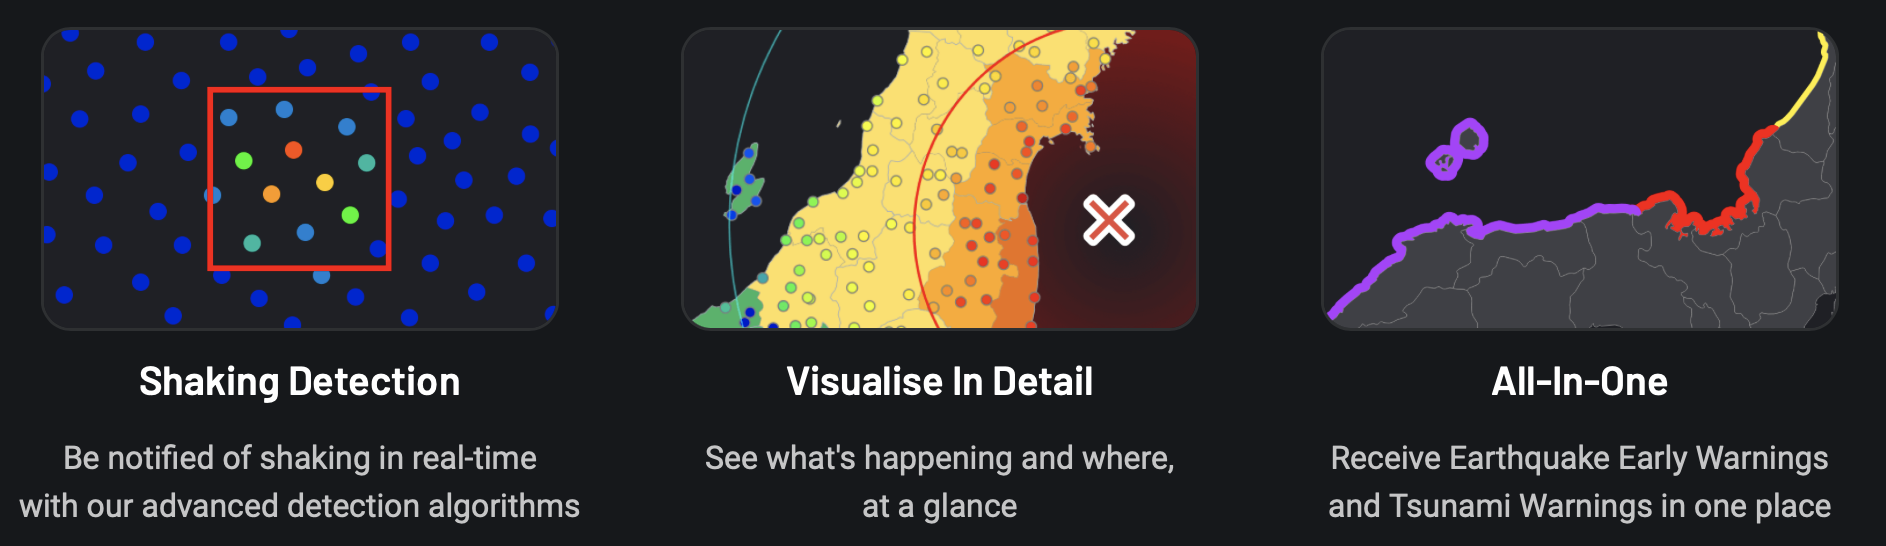
\includegraphics[width=0.6\linewidth]{jquake-features.png}
    \caption[Feature introduction of JQuake]{Feature introduction of JQuake, screenshot from website.}
    \label{fig:jquake-monitor-features}
\end{figure}

\begin{figure}[!ht]
    \centering

    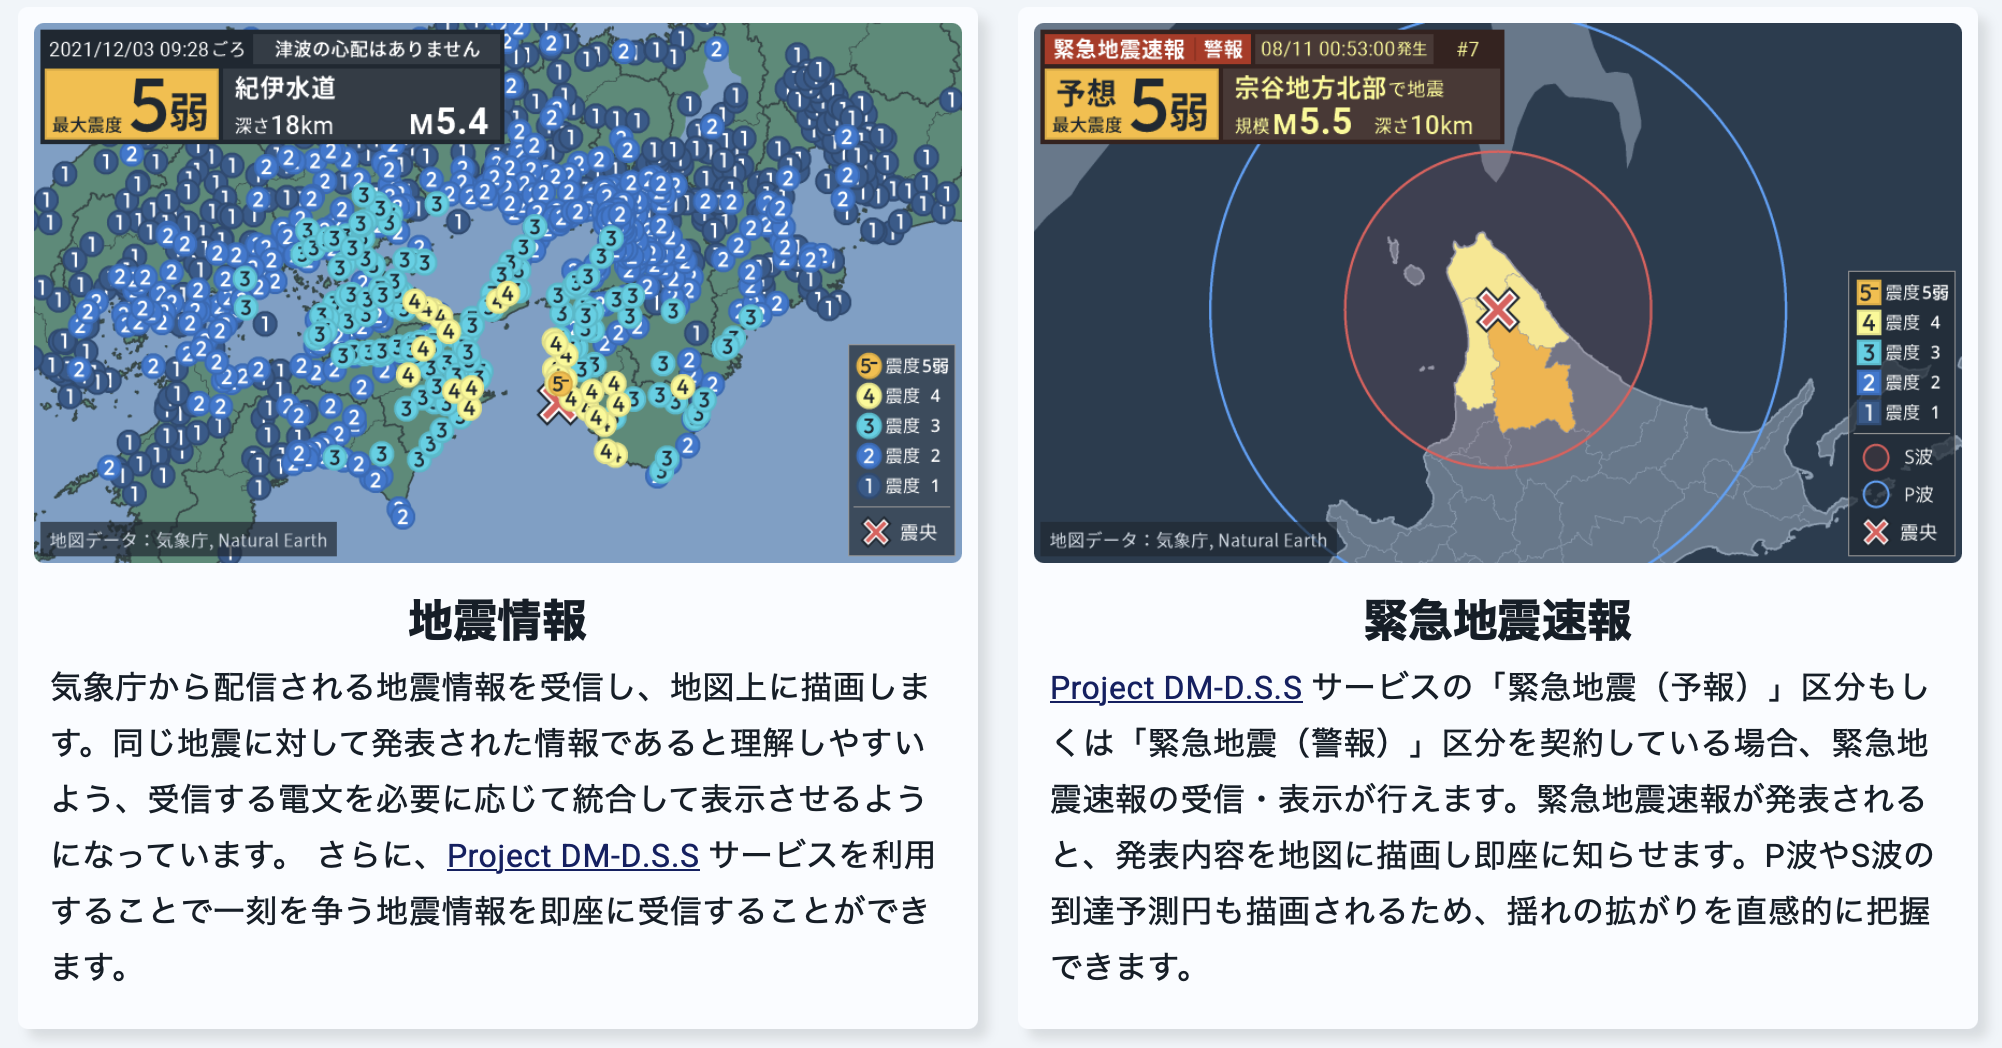
\includegraphics[width=0.6\linewidth]{quarog-features-1.png}\\
    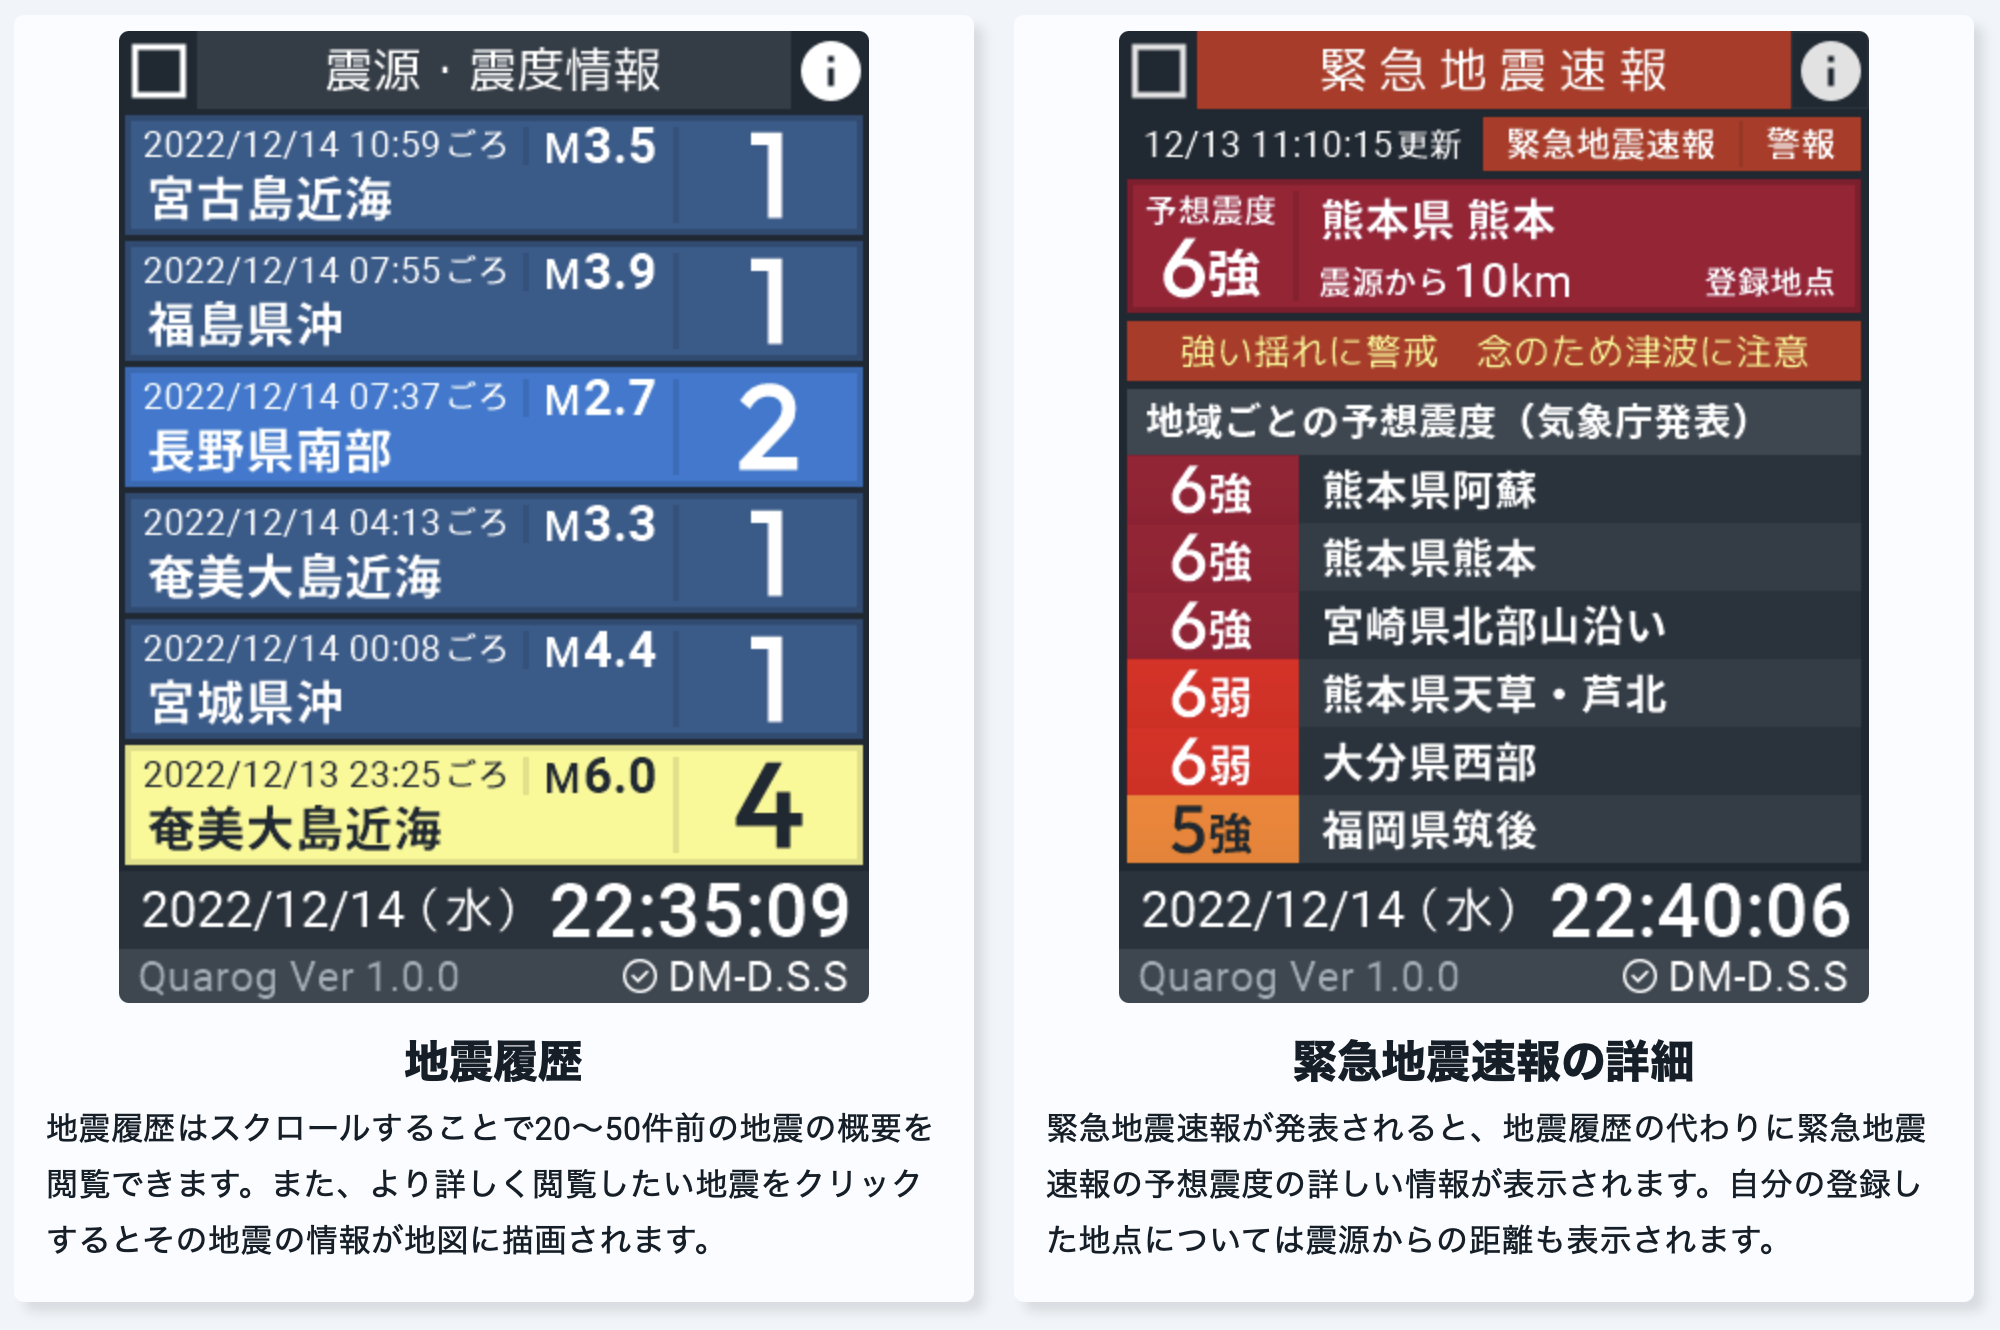
\includegraphics[width=0.6\linewidth]{quarog-features-2.png}
    \caption[Feature introduction of Quarog]{Feature introduction of Quarog, screenshot from website.\\Top-left: Past earthquake information; Top-right: Real-time EEW;\\Bottom-Left: Past earthquake list; Bottom-Right: Details of EEW.}
    \label{fig:quarog-monitor-features}
\end{figure}

There are also a variety of configuration options avaliable for all apps, as listed in Table \ref{table:exist-config}. Both KEV and Quarog supports the adjustment of the colour theme, and Quarog even supports changing the style of how blocks are displayed and coloured as shown in Figure \ref{fig:kev-colour-cust} and \ref{fig:quarog-cust}. Playing a sound on the speaker is also common among the apps to remind the user of earthquakes.

\begin{table}[!ht]
    \centering

    \begin{tabular}{|c||c|c|c|c|}
        \hline
        Feature             & JQuake     & SREV                                                   & KEV        & Quarog     \\
        \hline\hline
        DM-D.S.S. Login     & \checkmark & \footnote{Already integrated with special permission.} & \checkmark & \checkmark \\
        \hline
        Sound Alert         & \checkmark & \checkmark                                             & \checkmark & \checkmark \\
        \hline
        System Notification &            &                                                        & \checkmark &            \\
        \hline
        Colour Theme        &            &                                                        & \checkmark & \checkmark \\
        \hline
        Map Colouring Style &            & \checkmark                                             &            & \checkmark \\
        \hline
    \end{tabular}
    \caption{Feature comparison in configuration and customisability of existing solutions}
    \label{table:exist-config}
\end{table}

\begin{figure}[!ht]
    \centering

    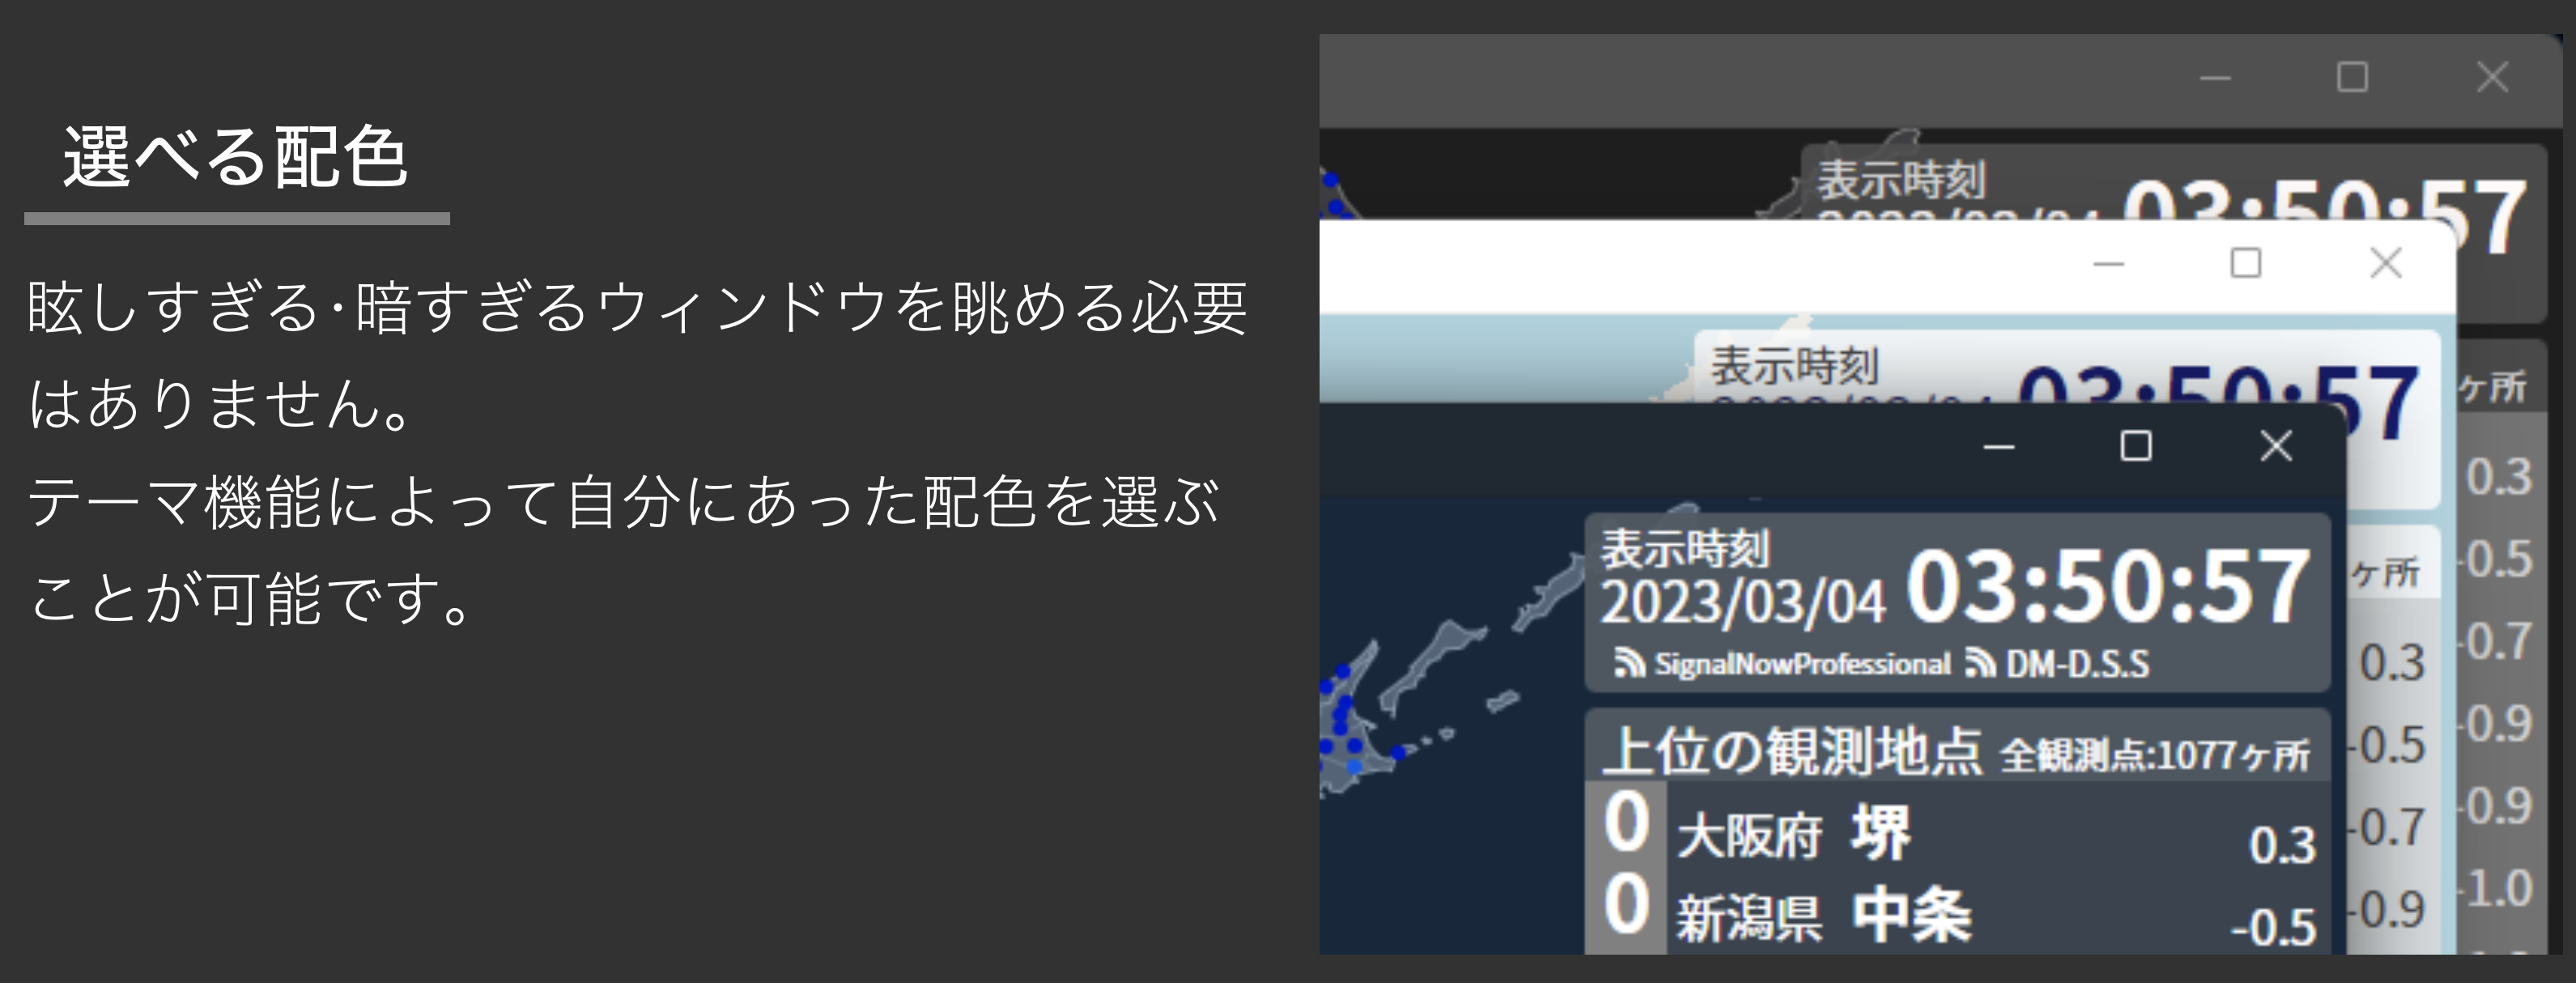
\includegraphics[width=0.5\linewidth]{kerv-colour.png}
    \caption[Customisable colour scheme of KEV]{Customisable colour scheme of KEV, screenshot from website.}
    \label{fig:kev-colour-cust}
\end{figure}

\begin{figure}[!ht]
    \centering

    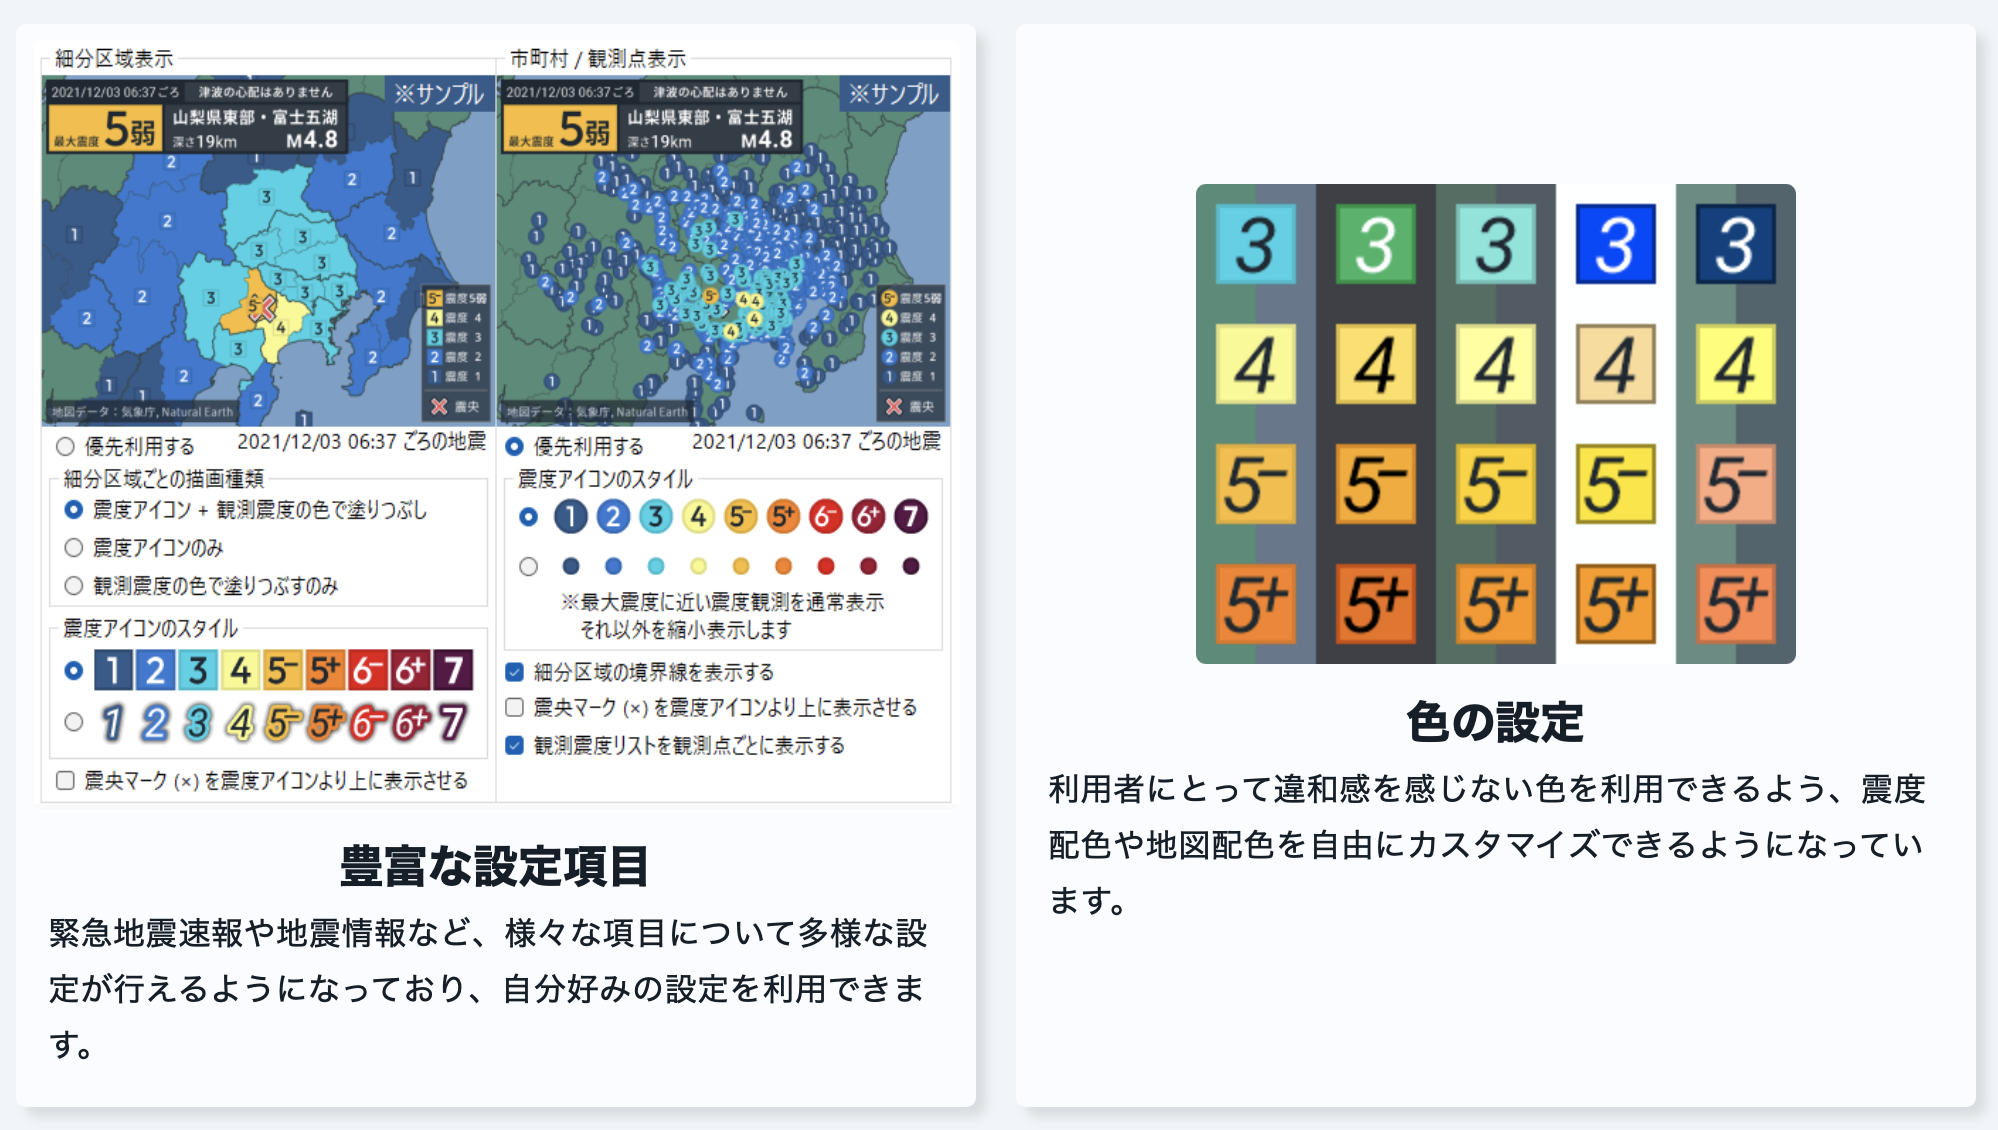
\includegraphics[width=0.6\linewidth]{quarog-cust.png}
    \caption[Customisablity of Quarog]{Customisablity of Quarog, screenshot from website.}
    \label{fig:quarog-cust}
\end{figure}

\subsection{Features of proposed solution}

Based on the potential user/client interview results, and the research into the exsisting solutions, the following key features should appear in the solution, since they are essential to earthquake monitoring applications:
\begin{enumerate}
    \item DM-D.S.S. Login functionality (for the data source)
    \item Real-Time Sensor Shake Internsity Data (w/ vibration alert)
    \item EEW Visuallisation (w/ Calculated Seismic Wavefronts)
    \item Past Earthquake List (w/ Option to review details)
    \item Tsunami Warning Visuallisation (w/ Related Sounds)
\end{enumerate}

However, due to the limitation of time and the difficulty of implementation, the following functionalities are not the key to implementation, which include mostly the customisation parts, ranked in decreasing importancy:
\begin{enumerate}
    \item User-Defined Key Monitor Point
    \item Customisable Sound Alert
    \item Customisable Colour Theme
    \item Customisable Map Colouring Style
\end{enumerate}

The following features might not be avaliable due to the time constraints and the complexity behind such system:
\begin{enumerate}
    \item Replay (due to a server needing to store past data)
    \item Sub-Map for the Okinawa Area (due to the difficulty in implementatino)
    \item Map Zooming Feature (due to the complexity in the map colouring functionality)
\end{enumerate}

With those key features implemented, the application should mirror all essential functionalities of a earthquake monitoring application, as compared to the four exsisting solutions above.

\subsection{Critical Path}

The functionality of this application can essentially be divied into \(1+2+1+n\) steps, where the 1 is to receive information from the API/Websocket provided by DM-D.S.S., and 2 is to, briefly say:
\begin{enumerate}
    \item Real-time Monitoring: Produce a real-time map to monitor real time vibration and plot real-time EEW/tsunami warnings
    \item Past-earthquake Viewing: Produce a menu to select an earthquake to display information on the map.
\end{enumerate}

The next 1 is to merge these two functions, specifically the functionality to switch back to the real-time monitoring option immediately when a new EEW is released (to make sure the user does not miss any information on realtime EEWs while looking at past earthquake information).

The final \(n\) is to implement a setting page for customisation.

TODO: Detailed Critical Path

\subsection{Requirements Specification}
The requirements specification is a document/contract with the client that outlines what you will deliver. The contents need to have SMART (specific, measurable, achievable, realistic, timely) goals.

After your system has been completed you will need to test against this.

\begin{table}[!ht]
    \centering

    \begin{tabular}{|l|p{0.15\linewidth}|l|p{0.3\linewidth}|}
        \hline
        Requirement \textnumero & Description & Success Criteria & Measurement Method \\
        \hline \hline
                                &             &                  &                    \\
        \hline
                                &             &                  &                    \\
        \hline
                                &             &                  &                    \\
        \hline
    \end{tabular}
    \caption{Table of Requirements.}
    \label{table:requirements}
\end{table}

\section{Design}
Algorithms + Data Structures = Programs.

\subsection{Hierarchy Chart}
A top-down approach to problem solving will lead to the identification of tasks with sub-tasks. i.e. modules and functions required. This shows how \textbf{decomposition} is applied.

\begin{figure}[!ht]
    \centering
    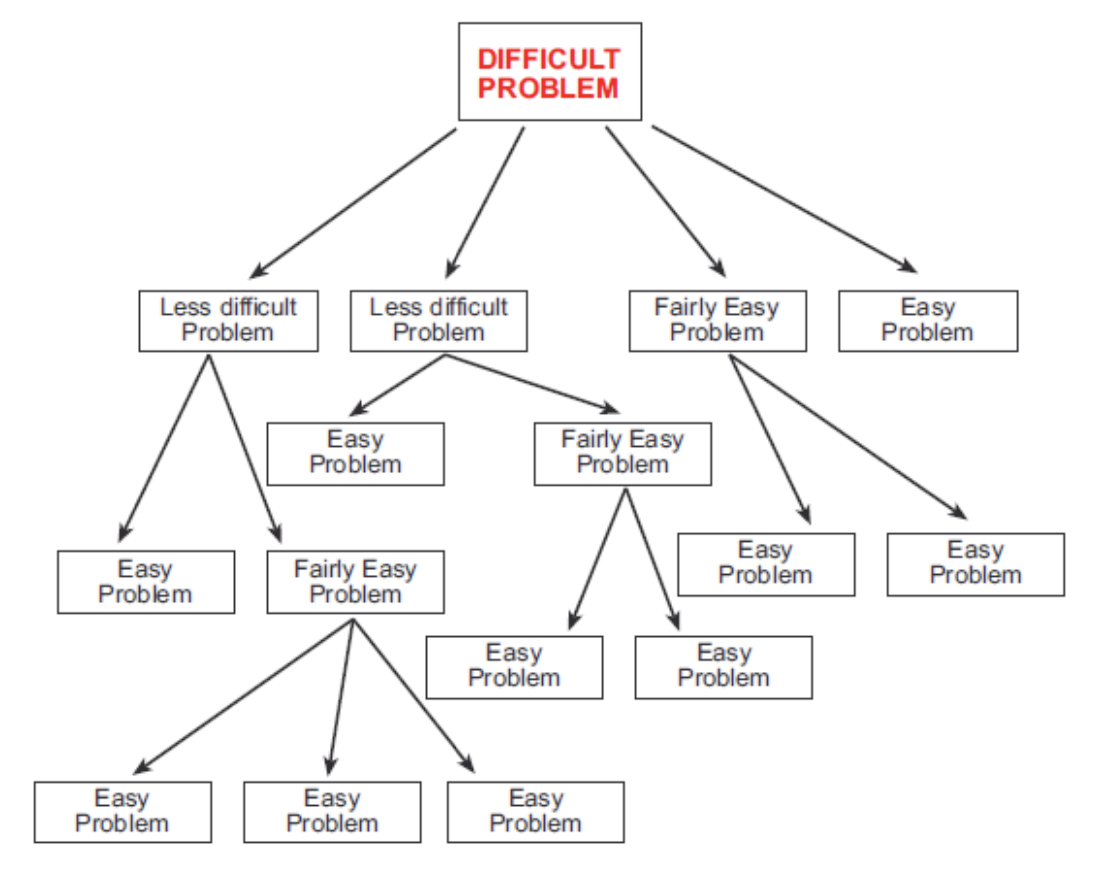
\includegraphics[width = 0.5\linewidth]{hierarchy_chart.png}
    \caption{Hierarchy Chart.}
    \label{fig:hierarchy}
\end{figure}

\subsection{Data Structures/Data modelling}
\subsubsection{External Data Sources}
If you are scraping/gathering data from APIs from external sources you should define the relevant format/parameters.

\subsubsection{OOP Model}
OOP modelling (classes, methods, attributes, inheritance etc.). Class diagrams would be useful (these are covered in Bond book 1 page 185 onwards). Diagrams should follow conventions for inheritance/composition and private/protected/public methods/attributes.

\begin{figure}[!ht]
    \centering
    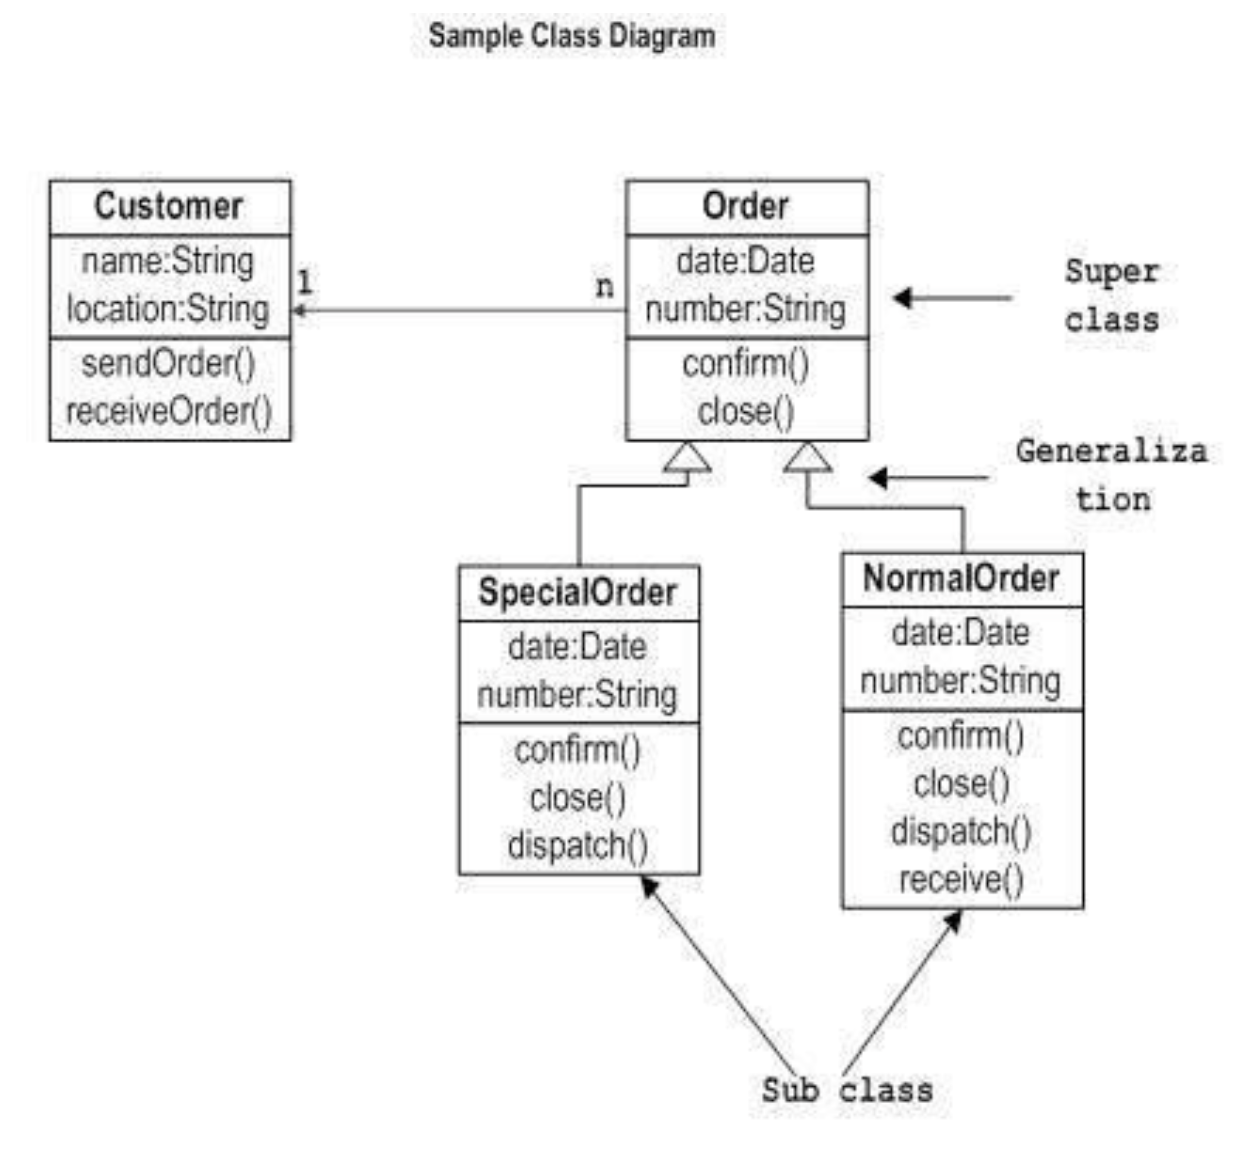
\includegraphics[width = 0.5\linewidth]{class_diagram.png}
    \caption{Class Diagram.}
    \label{fig:classes}
\end{figure}

\subsection{User Interface}
You will need to draw up a prototype for the user interface. You may do this within the software package you implement your solution in.
\begin{itemize}
    \item Screen designs
    \item Menu options/sequences
    \item Buttons/keys/commands (command line)
\end{itemize}

\subsection{Hardware \and Software Requirements}
Draw up a hardware and software specification for items that are required.

\section{Technical Implementation}
\subsection{Key Code Segments}
\subsubsection{Data structures}
Implementation of ADTs and OOP Classes to be demonstrated.

\subsubsection{Modularity}
Code should be created and tested in separate modules that are integrated later. Use sub-headings for each module, define the purpose of the module, and show unit testing of the module.

\subsubsection{Defensive Programming/Robustness}
Exception handling

\section{Testing}
Consider how you will test your project. You should devise a test strategy that encompasses a range of methods.

\subsection{Test Strategy}
\begin{itemize}
    \item Unit testing (of individual functions)
    \item Integration testing (e.g. different modules/class files)
    \item Robustness (demonstrating defensive programming skills/exception handling)
    \item Requirements testing (against your initial requirements - a table with test number, description, test data, expected result, evidence (screenshot/video time link) would be suitable)
    \item Independent end user beta testing (this will assist with your evaluation)
\end{itemize}

\subsection{Testing Video}
\begin{itemize}
    \item You can include a video to assist (but you will need to reference the timepoint at which relevant evidence appears)
    \item If you include a video you will need to have it publicly available.
    \item It is suggested that you include a QR code in your testing to give a link to it the video (for the moderator) rather than just giving a long URL on its own.
\end{itemize}

\subsection{System Tests (against original requirements specification)}
You need to give evidence in support of requirements that have been met e.g. reference to a relevant test/screenshot/relevant code.

\begin{table}[!ht]
    \centering

    \begin{tabular}{|l|p{0.15\linewidth}|l|p{0.3\linewidth}|}
        \hline
        Requirement \textnumero & Description & Success Criteria & Tests + Evidence \\
        \hline \hline
                                &             &                  &                  \\
        \hline
                                &             &                  &                  \\
        \hline
                                &             &                  &                  \\
        \hline
    \end{tabular}
    \caption{Table of Tests.}
    \label{table:tests}
\end{table}

\section{Evaluation}
\subsection{Requirements Specification Evaluation}
Personal evaluation
\begin{itemize}
    \item Copy and paste your original requirements from your project analysis
    \item You need to review each requirement and comment objectively on whether it was \textit{fully met/partially met/not met}.
\end{itemize}

\begin{table}[!ht]
    \centering

    \begin{tabular}{|l|p{0.15\linewidth}|l|p{0.3\linewidth}|}
        \hline
        Requirement \textnumero & Description & Success Criteria & Fully/Partial/Not met (Reflective Comment) \\
        \hline \hline
                                &             &                  &                                            \\
        \hline
                                &             &                  &                                            \\
        \hline
                                &             &                  &                                            \\
        \hline
    \end{tabular}
    \caption{Table of Evaluation.}
    \label{table:evaluation}
\end{table}

\subsection{Independent End-User Feedback}
End user/client evaluation
\begin{itemize}
    \item there \textbf{must} be meaningful end user feedback
    \item You should hold a review meeting with your end user
    \item Write down any key feedback that they give you. E.g. Agreement that a particular requirement has been meet/comments as to aspects that they find sub-optimal/comments as to additions they would like to see
\end{itemize}

\begin{table}[!ht]
    \centering

    \begin{tabular}{|l|p{0.15\linewidth}|l|p{0.3\linewidth}|}
        \hline
        Requirement \textnumero & Description & Acceptance Y/N & Additional Comments \\
        \hline \hline
                                &             &                &                     \\
        \hline
                                &             &                &                     \\
        \hline
                                &             &                &                     \\
        \hline
    \end{tabular}
    \caption{Table of Feedback.}
    \label{table:feedback}
\end{table}

\subsection{Improvements}

You need to give consideration to a number of potential future improvements that could be made. They may arise from either your experience or from feedback given to you by your end user. Ideally at least one should be in response to end user feedback.

\begin{itemize}
    \item Write a paragraph for each potential improvement/change
    \item The improvements/changes could result from additional functionality that has been identified as being beneficial or could be as a result of required efficiencies if some processes are clunky or require faster run-times
    \item You should then comment on how the proposed change could be implemented moving forward. i.e. what would need to be changed/developed and how? You are not expected to actually make any changes; just comment on the possibilities.
\end{itemize}

\section{Code Listing}

\newpage
\listoftables
\listoffigures
\end{document}